\chapter{Numerical methods to simulate dispersed phase}
	\label{ch3:disperse_phase_methods}

\section{Introduction}

The previous chapter presented numerical methodologies applicable to separate two-phase flows. Such methods are useful for solving problems where the dynamics of atomization need to be accurately resolved. Nonetheless, these are not suitable to tackle dispersed phase problems due to the high computational costs involved in resolving and transporting a spray composed of many droplets. Furthermore, resolved atomization methods are not able to efficiently solve for multiphysics phenomena relevant in combustion systems such as evaporation, being an ongoing research line nowadays \citepColor[boniou_numerical_2022]. Therefore, dispersed-phase regimes need a different representation of the liquid phase so that: 1) the spray can be transported with acceptable computational costs and 2) more complex physics relevant to reactive problems can be included, such as evaporation and combustion.

In this chapter, numerical strategies to simulate dispersed phase flows are reviewed. Section \ref{sec:ch3_numerical_approaches_dispersed_phase} summarizes some of the available formalisms that can be chosen for solving a dispersed phase problem, with special emphasis on the lagrangian point-particle approach which is employed in this thesis. Then, section \ref{sec:ch3_state_art_lagrangian_injection} presents the state of the art on lagrangian methods to simulate fuel injection in MSFI systems, which is the starting point of this work.

\section{Numerical approaches to model dispersed phase flows}
\label{sec:ch3_numerical_approaches_dispersed_phase}


The spray generated in the dispersed phase regime is mainly distinguished from liquid in the separate regime by the following features (represented in Figure \ref{fig:atomization_regimes_herrmann}):

\begin{itemize}

	\item The characteristic length scales of the particles. In dispersed phase flows, these ones are usually smaller than the resolution of the main grid.
	
	\item The value of the liquid volume fraction $\alpha_l$. In dispersed phase flows, $\alpha_l < 1$. According its value, one can distinguish between dense regime (moderate values of $\alpha_l$, particles are close to each other) and dilute regime (lower values of $\alpha_l$, usually below $10^{-3}$, particles are far from each other).

\end{itemize}

The numerical formalisms to resolve dispersed phase flows will hence depend on these two characteristics. It is also important to consider the interaction with the gaseous phase, since its resolution depends on the main grid. The interaction between the liquid and gaseous phases in dispersed phase flows can be quantified by means of the Stokes number $St$, defined as the ratio between the characteristic time-scale of a liquid particle $\tau_p$ and a characteristic time of the gaseous phase $\tau_g$: 

\begin{equation}
\label{eq:Stokes_number_definition_general}
St = \frac{\tau_p}{\tau_g}
\end{equation}

A classification of numerical methods to simulate dispersed phase flows based on the volume fraction and the Stokes number has been done by \citeColor[balachandar_scaling_2009], shown in Figure \ref{fig:balachandar_numerical_methods_representation}. As it can be seen, the Stokes number will depend on the numerical methodology used to resolve the gaseous phase: in DNS, the smallest scales of turbulence with characteristic size $\upeta$ will be resolved and will have a characteristic time $\tau_k$, while in LES the smallest scales resolved $\upxi$ will be larger and their time-scales will be different ($\tau_\upxi$). Regarding the volume fraction, coupling strategies between liquid particles and gas can be used depending on its value: in the dilute regime particles are far from each other and the interactions among them can be neglected (one and two-way coupling), while in the dense regime the interaction between particles must be taken into account (four-way coupling). The difference between one and two-way coupling depends on if the influence of the liquid phase onto the gas is considered with source terms (two-way coupling) or if it is neglected, so that the gaseous phase will not be perturbed by the particles (one-way coupling).


\begin{figure}[h!]
	\centering
	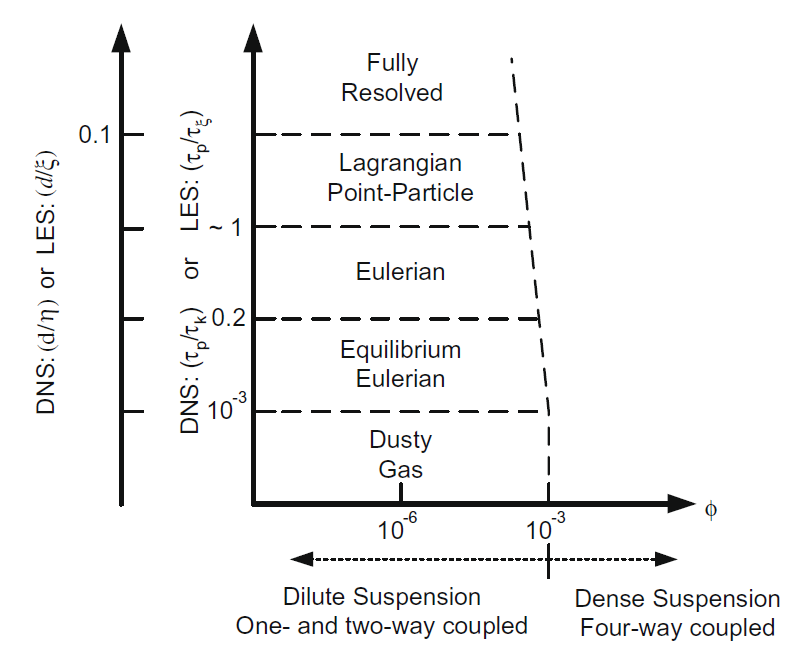
\includegraphics[scale=0.6]{./part1_numerical_approaches/figures_ch3/balachandar_disperse_phase_classification}
	\caption[Numerical approaches to solve dispersed phase flows]{Numerical approaches to solve dispersed phase flows. Classification is done with respect to the liquid volume fraction (here defined as $\phi$) and to the Stokes number or, equivalently, to the ratio of largest to smallest length scales, which depend on the numerical resolution.  Source: \citeColor[balachandar_scaling_2009]}
	\label{fig:balachandar_numerical_methods_representation}
\end{figure}

%The different dispersed phase methodologies aim at resolving Eq. (\ref{eq:WBE_spray_representation}), either by approximating this equation to obtain the function $f$ or by making point-particles assumptions, as shown in Figure \ref{fig:balachandar_numerical_methods_representation}. This chapter makes a review of some of these strategies, with special emphasis on the lagrangian point-particle approach which is employed in this thesis.


\subsection{Statistical methods}
\label{subsec:ch3_statistical_methods}

A spray composed of dispersed droplets can be characterized by means of a number density function $f$. This function depends on time $t$, space $\textbf{x}$, velocity $\textbf{u}$ and radius $r$, and can be expressed as follows \citepColor[subramanian_statistical_2000]:

\begin{equation}
\label{eq:f_spray_description_subramanian}
f \left( t, \textbf{x}, \textbf{u}, r \right) = \sum_{p=1}^{N_d} \delta \left( \textbf{x} - \textbf{x}_p \left( t \right) \right)  \delta \left( \textbf{u} - \textbf{u}_p \left( t \right) \right) \delta \left( \textbf{r} - \textbf{r}_p \left( t \right) \right)
\end{equation}

where $N_d$ is the number of droplets in the spray, and $\textbf{x}_p$, $\textbf{u}_p$ and $r_p$ are each individual particles position, velocity and radius respectively. The function $f$ contains all the necessary information to represent the spray. This function is governed by a William-Boltzmann Equation \citepColor[williams_spray_1958]:

\begin{equation}
\label{eq:WBE_spray_representation}
\frac{\partial f}{\partial t} + \nabla_{\textbf{x}_p} \left( \textbf{u}_p f \right) + \nabla_{\textbf{u}_p} \left( \textbf{F}_p f \right) + \frac{\partial E_{S_p} f}{\partial S_p} + \frac{\partial E_{T_p} f}{\partial T_p}
\end{equation}

where $\textbf{x}_p$, $\textbf{u}_p$, $S_p$ and $T_p$ are each individual particle's position, velocity, surface and temperature, respectively; $\textbf{F}_p$ is the force acting on the particle, and $E_{S_p}$ and $E_{T_p}$ are respectively the exchange terms due to mass (evaporation rate) and energy (heat transfer). Statistical approaches aim at determining the function $f$ by solving/approximating Eq. (\ref{eq:WBE_spray_representation}). Stochastic methods to solve for the dispersed phase include the stochastic lagrangian approach of \citeColor[dukowicz_particle-fluid_1980], eulerian methods considering a monodisperse \citepColor[drew_theory_1999] or a polydisperse spray \citepColor[laurent_multi-fluid_2001], and quadrature methods. These methods are out of the scope of the present work and hence are not discussed here.



\subsection{Eulerian methods}

Eulerian methods, also called Euler-Euler formalism (EE), are widely used to model dispersed two-phase flows. The same grid is used for resolving both the carrier and dispersed phases. The carrier phase is solved from the Navier-Stokes equations ($\S$\ref{sec:ch2_governing_equations}) applied to the gas. For characterizing the dispersed phase, averaged properties and statistical tools are used. These methods present, however, difficulties when dealing with the polydispersion of the spray and when modeling the particles collisions and interactions with the walls \citepColor[garcia_developpement_2009].

To solve for the dispersed phase, a well-known eulerian formalism is the mesoscopic approach. The particles are described according to the kinetic theory of gases formulated by \citeColor[chapman_mathematical_1970], so that mesoscopic variables are used to get averaged properties of the spray. In order to develop the equations for the dispersed phase, several assumptions need to be made \citepColor[lancien_etude_2018]:

\begin{enumerate}

\item The atomization process is complete, particles are perfectly spherical and non-deformable.

\item The only force exerted by the carrier phase on the droplets is drag.

\item Temperature is homogeneous inside each droplet.

\item Spray is dilute: $\alpha_l < 10^{-2}$.

\item The interactions between droplets are neglected.

\item The spray is mono-disperse and mono-kinetic: at one point in time and space, the droplets all have the same diameter and velocity.

\item Similarly, at one point in time and space, all droplets have the same temperature.

%\item Random uncorrelated motion is neglected.

\end{enumerate}

With these assumptions, the dispersed phase is represented by the following equations based on statistical averages of the spray \citepColor[lancien_etude_2018]:

\begin{subequations}
\label{eq:EE_disperse_phase}
\begin{align}
\frac{\partial \overline{n}_l}{\partial t} + \nabla \left( \overline{n}_l \overline{\textbf{u}}_l \right)  &= 0 \\
\frac{\partial \rho_l \overline{\alpha}_l}{\partial t} + \nabla \left( \rho_l \overline{\alpha}_l \overline{\textbf{u}}_l \right) &= - \Gamma \\
\frac{\partial \rho_l \overline{\alpha}_l \overline{u}_{l,i}}{\partial t} + \nabla \left( \rho_l \overline{\alpha}_l \overline{\textbf{u}}_l \overline{u}_{l,i} \right) &= F_{d,i} - \overline{u}_{l,i} \Gamma  + \nabla \overline{\overline{\pmb{\tau}}}_l^{sgs} \\
\frac{\partial \rho_l \overline{\alpha}_l \overline{h}_l}{\partial t} + \nabla \left( \rho_l \overline{\alpha}_l \overline{\textbf{u}}_l  \overline{h}_l \right) &=  - \overline{h}_l  \Gamma + \overline{\Phi}
\end{align}
\end{subequations}

where $n_l$ is the number density of the particles, $\Gamma$ the evaporation rate, $F_{d}$ the drag force, $\overline{\overline{\pmb{\tau}}}_l^{sgs}$ the subgrid tensor of the liquid phase, $\overline{h}_l$ the liquid enthalpy and $\overline{\Phi}$ the conduction flux term. The exchange between phases is taken into account by the right hand sides of the previous expressions. As it is observed, multiphysics phenomena such as mass exchange due to evaporation and energy transfer can be taken into account with the corresponding exchange terms.  This is one of the advantage of the dispersed phase modeling of two-phase flows as opposed to the fully-resolved atomization methods presented in Chapter \ref{ch2:numerical_methods_resolved_atomization}.  Other frequently used Eulerian method is the Euler-Lagrange Spray Atomization (ELSA) model \citepColor[andreini_development_2016], which has also been coupled to resolved atomization simulation in the dense phase for solving more accurately atomization \citepColor[anez_multi-scale_2019].

\subsection{Lagrangian point particle representation}
\label{sec:ch3_EL_formalisms}

Another well-know methodology to simulate dispersed phases systems, broadly employed in aerospace applications, is the lagrangian point particle (LPP) representation. In this formalism, the gas is resolved in the main eulerian grid, but the particles conforming the dispersed phase are tracked individually and represented by a different set of equations. Since the carrier phase is solved in an eulerian grid and the dispersed phase is modeled separately, these method is usually referred as the Euler-Lagrange (EL) formalism. This can make convergence difficult and hinders the introduction of parallelism techniques. As advantages, the resulting the time per iteration is usually lower than for the EE description, and the drop-drop and drop-wall interactions are easier to model.

\subsubsection*{Dynamics of liquid particles}

For describing particles in the lagrangian framework, each particle will be modeled according to the \textbf{Discrete Particle Simulation} (DPS) approach. In DPS, liquid particles are completely spherical, robust, and defined spatially as points, so that the location of each parcel can be represented by a single position vector. With these assumptions, the \textbf{dynamic equations} for a particle $p$ are \citepColor[maxey_equation_1983]:

\begin{subequations}
\label{eq:TPF_lagrange_dynamic_eqs}
\begin{align}
\frac{d \boldsymbol{x}_p}{d t} &= \boldsymbol{u}_p \\
\frac{d \boldsymbol{u}_p}{d t} &= \underbrace{ - \frac{3}{4} \frac{\rho_\mathrm{g}}{\rho_p} \frac{C_D}{d_p} | \boldsymbol{v}_r | \boldsymbol{v}_r }_{\text{Drag}\atop\text{term}}  + \underbrace{ \left( 1 - \frac{\rho_\mathrm{g}}{\rho_p} \right) \boldsymbol{g} }_{\text{Gravity}\atop\text{term}} 
\end{align}
\end{subequations}

where $\textbf{x}_p$ and $\textbf{u}_p$ are the position and velocity of the particle, $\textbf{v}_r = \boldsymbol{u}_p  - \boldsymbol{u}_g$ the relative velocity between the particle and the gas, $\rho_\mathrm{g}$ and $\rho_p$ are the gas and liquid particle densities, $C_D$ a drag coefficient, and $d_p$ the particle diameter. Equation (\ref{eq:TPF_lagrange_dynamic_eqs}b) is the momentum equation of the droplet and contains the contributions of the two forces considered: the drag forces and the gravitational forces. The first ones are usually the main mechanism of momentum transfer between phases, while the latter are often several orders of magnitude smaller and can usually be neglected (specially at high speeds, where drag dominates the momentum transfer). 

The drag coefficient of the particles $C_d$ can be evaluated with the following expression, obtained experimentally by \citeColor[schiller_drag_1935]:

\begin{equation}
\label{eq:Re_CD_droplet}
C_D =
\left\{
    \begin{split}
     \frac{24}{Re} \left( 1 + 0.15 Re^{0.687} \right)\,\,\mathrm{if}\,\,Re < 1000 \\ 
    0.44\,\,\mathrm{if}\,\,Re \geq 1000 
    \end{split}
\right.
\end{equation}

where $Re = \rho_\mathrm{g} | \boldsymbol{v_r} | d_p / \mu_\mathrm{g} $ is the Reynolds number based on the relative velocity and particle diameter. \\

When considering a lagrangian approach, the influence of the carrier phase on the liquid particles will have a determining effect on their motion. This influence can be quantified by means of the Stokes number defined previously by Eq. (\ref{eq:Stokes_number_definition_general}). Its magnitude indicates how the droplet responds to fluctuations of the gas flow. If $St << 1$, the droplet will follow perfectly the fluctuations of the gas flow. On the contrary, if $St >> 1$ the droplets will rather neglect the flow trajectories and follow its own track (ballistic behaviour). 

For evaluating the Stokes number, the characteristic timescale for each phase need to be determined. The gaseous timescale can be determined as $\tau_g = d_p / | \textbf{u}_p |$. Particle timescales can be estimated from the following expression \citepColor[maxey_equation_1983]:

\begin{equation}
\tau_p = \frac{d_p^2 \rho_p}{18 \mu_\mathrm{g}} =  \frac{4}{3} \frac{\rho_p}{\rho_\mathrm{g}} \frac{d_p}{C_D | \boldsymbol{v}_r |} = \frac{4}{3} \frac{\rho_p d_{p^2}}{\mu_g Re C_D}
\end{equation}

which can be seen as the relaxation time of the particle; in other words, the time that one particle takes to respond to the fluctuations in the velocity field.


\subsubsection*{Coupling with mass and energy transfer}

As in the EE method, the LPP representation also allows to couple the dynamic equation with exchange terms for mass and energy transfer with the gaseous phase:

\begin{subequations}
\label{eq:TPF_lagrange_phasetransition_eqs}
\begin{align}
\frac{d m_p}{d t} &= \dot{m}_p = \Gamma \\
\frac{d h_p}{d t} &= m_p C_{P_\mathrm{g}} \frac{d T_p}{d t} = \Phi
\end{align}
\end{subequations}

where $m_p$, $h_p$, $T_p$ and $C_{P_\mathrm{g}}$ are respectively the particle mass, enthalpy, temperature and gas specific heat capacity at constant pressure. $\Gamma$ and $\Phi$ are the corresponding source terms for mass and energy. It follows that Equation (\ref{eq:TPF_lagrange_phasetransition_eqs}a) accounts for the \textbf{evaporation} process. If a single component is considered and the uniform temperature model for evaporation is used \citepColor[abramzon_droplet_1989], then the evaporation term can be expressed as:

\begin{equation}
\Gamma = - \pi d_p Sh \left( \rho_p D_F \right) \ln \left( 1 + B_M \right)
\end{equation}

where $Sh$ is the Sherwood number, $D_F$ the fuel diffusivity, and $B_M$ the Spalding mass number. \\

For evaluating the energy transfer in the droplets, the physical processes of \textbf{conduction} and  \textbf{evaporation} are taken into account. Then, the source $\Phi_p$ is obtained from the following energy balance.

\begin{equation}
\Phi_p = \underbrace{ h_p \pi d_p^2 \left( T_\mathrm{g} - T_p \right) }_{\text{Conduction}\atop\text{term}} - \underbrace{ \dot{m}_p  \Delta h_v }_{\text{Evaporation}\atop\text{term}}
\end{equation}

where $T_\mathrm{g}$ is the gas temperature, $h_p$ is the film coefficient of the gas at the particle surface and $\Delta h_v$ is the latent heat of vaporization of the particle. Eqs. (\ref{eq:TPF_lagrange_phasetransition_eqs}) can be solved together with Eqs. (\ref{eq:TPF_lagrange_dynamic_eqs}) to obtain the evolution of mass and energy of the droplets with time as they move within the carrier phase.

\section{Stage of the art in injection models for MSFI systems}
\label{sec:ch3_state_art_lagrangian_injection}

Several numerical formalisms for modeling the dispersed phase in two-phase flows have been introduced in the previous section. In this work, the lagrangian representation presented in $\S$\ref{sec:ch3_EL_formalisms} is used to model the dispersed phase due to its low computational cost and its applicability to account for polydispersity of the spray.%, which is of particular interest to develop realistic lagrangian injectors as stated in $\S$\ref{sec:ch1_objective_thesis_outline}.

In all dispersed-phase simulations, the first step is to introduce the lagrangian droplets in the domain with their proper boundary conditions. This is achieved by means of \textbf{lagrangian injection models}, which are the main interest of the present work. The fact of using a lagrangian approach for representing the particles has the advantage of allowing the injection of a polydisperse spray from the beginning of the simulation, something which is not possible with other dispersed formalisms such as the eulerian ones. This is of particular interest for performing injection in realistic systems, such as in MSFI configurations presented in $\S$\ref{sec:ch1_fuel_injection_technology}. 

This section presents the state of the art in models for lagrangian injection with particular focus on MSFI systems. Figure \ref{fig:state_art_injection} proposes a classification for existing models in literature grouped in a Venn diagram, distinguishing five categories and their interactions. Each research work is located according to the characteristics of the model employed, and the configuration of application within the MSFI models (hollow cone, airblast and JICF) is also specified. Several models are \textbf{based on empirical laws} obtained from experimental works, with the main advantage that the physics of the problem are already embedded in these laws, but on the other hand restricted to applications with identical geometry and operating conditions as in the test. Regarding the size of injected droplets, it is found that the \textbf{injection of a fully developed spray}, often obtained from experiments providing the spray granulometry further downstream the injection nozzle where atomization is fully complete, is usually performed. In the sense of droplet transport, it is sometimes necessary to consider the \textbf{effect of the dense spray on the gaseous phase}: in some configurations (especially in the JICF), coherent structures of the dense regime where primary atomization takes place might perturb the gaseous flow which will consequently affect the convection of droplets further downstream. Since the dense regime is neglected in lagrangian computations, this liquid-gas interaction is not directly taken into account, so the droplet transport might not be well resolved. Furthermore,  \textbf{secondary breakup of particles} in lagrangian simulations can be considered by means of secondary atomization models. This is specially useful in models which do not inject a developed spray, as the initial droplets will have a larger size than the diameters found in the equivalent real configuration. Independently of evaporation, the decrease of droplets size up to a value which is at equilibrium with the surrounding air can be accounted for with these models.

At last, a category called \textbf{reference spray learning} is present in Figure \ref{fig:state_art_injection}. It includes models that can use a reference spray to learn its characteristics (droplets sizes, velocity distributions and injection location) and impose realistic spray boundary conditions in dispersed phase simulations. As main advantage, such models could be applied to a wide range of injector configurations and operating conditions. Nevertheless, they require a proper characterization of the spray coming from simulations or experiments. This thesis aims at providing a numerical methodology for developing injection models that are able to follow this reference spray learning process. These models are explained in Chapter \ref{ch4:sli_development}, so they will not be further discussed in this section. The next lines are then devoted to explain some of the injection models in Figure \ref{fig:state_art_injection} which are of interest for MSFI systems, whose main mechanisms of injection are shown in Figure \ref{fig:multipoint_injector_snecma}.

%Each category has the following advantages and disadvantages (see presentation 2020 12 15):
%
%\begin{itemize}
%
%	\item \textbf{Based on empirical laws}. \textcolor{green}{Advantage}: embedded physics. \textcolor{red}{Disadvantage}: restricted to geometry and operating conditions of development.
%	
%	\item \textbf{Injection of fully developed spray}. \textcolor{green}{Advantage}: droplets size distributions directly imposed. \textcolor{red}{Disadvantage}: Primary atomization neglected.
%	
%	\item \textbf{Effect of dense spray in gaseous phase}. \textcolor{green}{Advantage}: in JICF, taking into account blockage effect. \textcolor{red}{Disadvantage}: None.
%	
%	\item \textbf{Addition of secondary atomization model}. Good if atomziation not present.
%	
%	\item \textbf{Reference spray learning}. So far, and to our knowledge, there are no available models that can use a reference spray to learn boundary conditions (droplet sizes, velocity distributions, spatial location of injectors) for dispersed phase computations. \textcolor{green}{Advantage}: Applicable to generic injectors and 
%	wide range of operating conditions.  \textcolor{red}{Disadvantage}: Need of detailed spray characterisation from simulations or experiments.
%
%\end{itemize}

%\begin{figure}[h!]
%	\centering
%	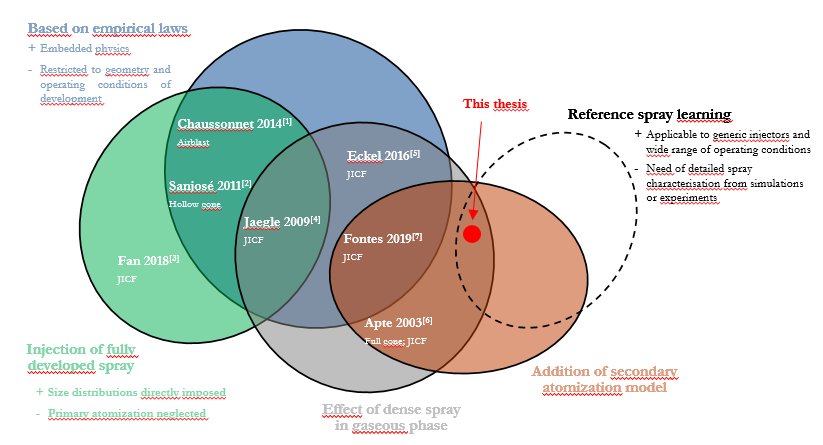
\includegraphics[scale=0.5]{./part1_numerical_approaches/figures_ch3/state_art_lagrangian}
%	\caption{Classification of lagrangian injection models}
%	\label{fig:state_art_injection}
%\end{figure}

\begin{figure}[h!]	
	\centering
	\includeinkscape[inkscapelatex=true,scale=0.70]{./part1_numerical_approaches/figures_ch3/state_art_lagrangian}
	\caption{Classification proposed for the state of the art in lagrangian injection modeling.}
	\label{fig:state_art_injection}
\end{figure}

\subsection{Hollow cone spray}
\label{subsec:ch3_hollow_cone_spray}

Pressure-swirl atomizers for delivering fuel through the pilot stage in multi-staged injectors will create a hollow cone spray. An example of pressure-swirl injector is shown in Figure \ref{fig:hollow_cone_view}: liquid is injected inside the nozzle with a rotational component (swirl), that will eventually create a hollow cone when the fuel leaves the nozzle. These type of nozzles are widely used and have been extensively studied both experimentally and numerically. Several models exist in literature for modeling the fuel injection in pressure-swirl with lagrangian formalisms. In this section two models are presented: the FIM-UR methodology developed by \citeColor[sanjose_fuel_2011], and the LISA model presented in \citeColor[guedot_developpement_2015].

\begin{figure}[ht]
    \centering
    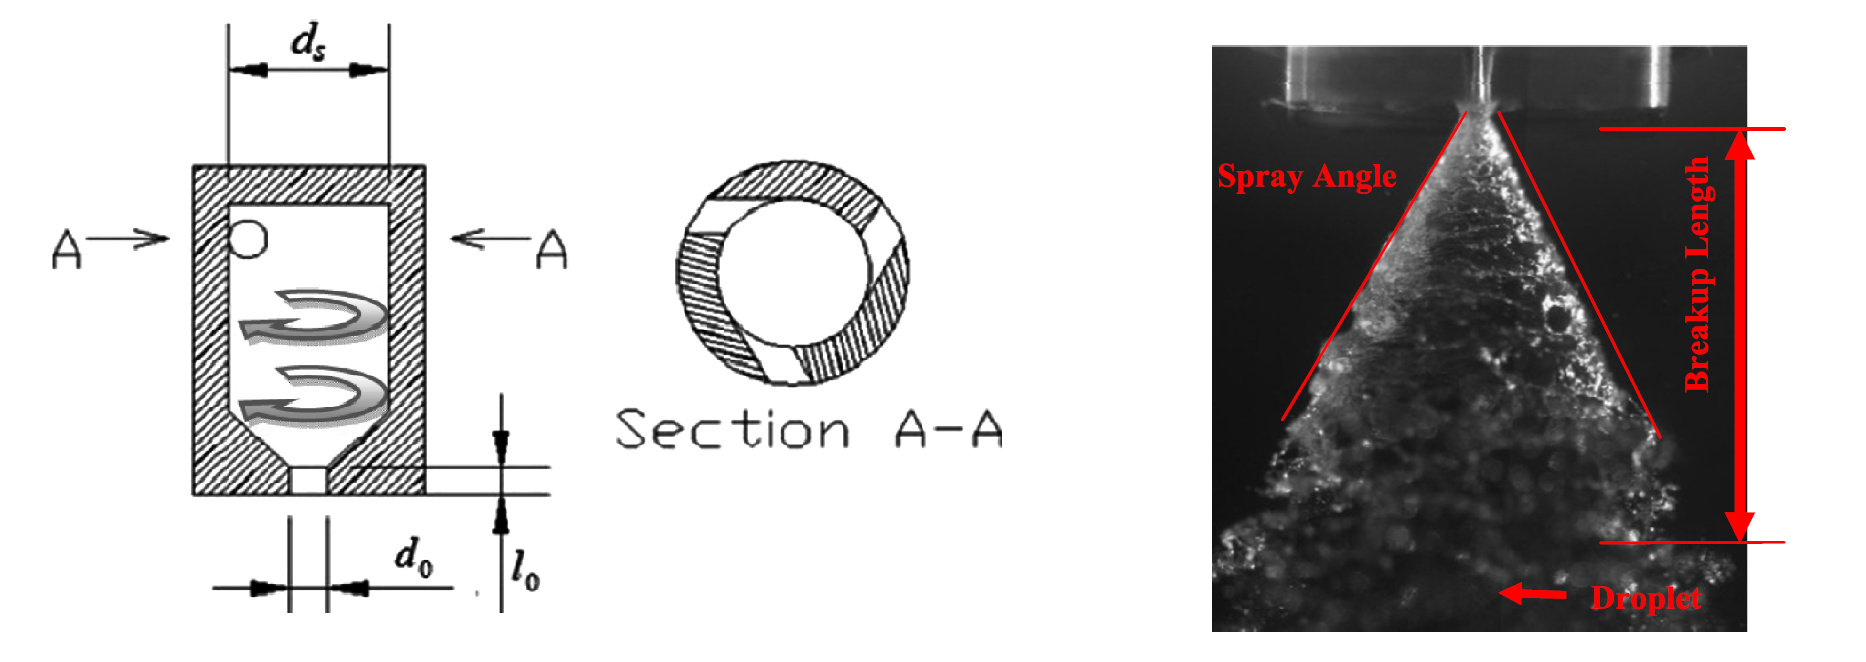
\includegraphics[width=0.8\textwidth]{./part1_numerical_approaches/figures_ch3/pressure-swirl-atomizer-wei}
       \centering
    \caption[Pressure-swirl atomizer]{Pressure-swirl atomizer.  \textsl{Left}: schematical view. \textsl{Right}: experimental snapshot with key hollow-cone spray features. Source: \citeColor[wei_improved_2014].}
    \label{fig:hollow_cone_view}
\end{figure}







\subsubsection*{FIM-UR model}

Fuel Injection Model by Upstream Reconstruction (FIM-UR) is an injection model which prescribes a developed spray in pressure-swirl atomizers, neglecting the atomization process. In its original formulation by \citeColor[sanjose_fuel_2011], a monodisperse spray is imposed. The extension to polydisperse sprays has been done by \citeColor[vie_accounting_2013].


\begin{figure}[ht]
    \centering
    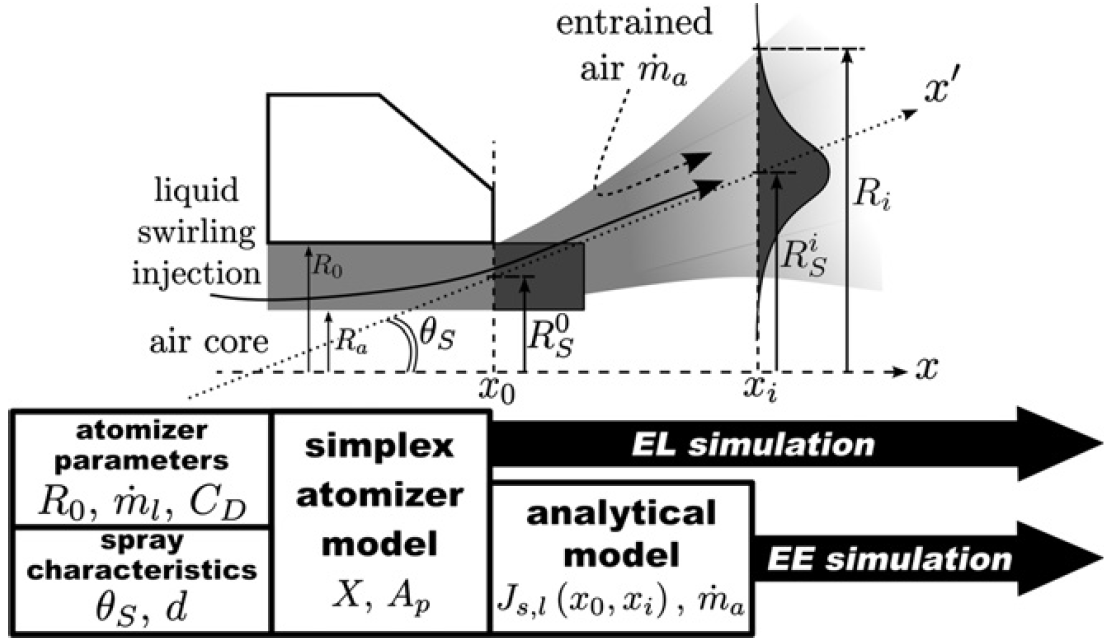
\includegraphics[width=0.7\textwidth]{./part1_numerical_approaches/figures_ch3/FIMUR}
       \centering
    \caption[FIMUR model for injection in pressure-swirl atomizers]{FIMUR model for injection in pressure-swirl atomizers. Source: \citeColor[sanjose_fuel_2011].}
    \label{fig:FIMUR_methodology}
\end{figure}

The principles of FIM-UR are shown in Figure \ref{fig:FIMUR_methodology}. The spray is imposed at an injection location $x_i$, whose boundary conditions are obtained by reconstruction from the properties at the real injection location $x_0$. FIM-UR can be applied for both EL and EE simulations, with the difference that the latter require additional analytical calculations to determine the momentum transfer and the entrained air mass flow rate. Both cases use the same model inputs: the spray is characterized by the diameter of droplets $d$ and the half-spray mean angle $\theta_s$, and the atomizer is parametrized by its exit radius $R_0$ and the injected liquid mass flow rate $\dot{m}_l$. Then, empirical formulas for pressure-swirl atomizers are used to calculate the remaining parameters of the model. The ratio $X$ of the air core surface $A_a$ to the discharge orifice surface $A_o$, called the contraction ratio, is given by \citeColor[rizk_internal_1985]:

\begin{equation}
X = \frac{A_a}{A_0} = \left( \frac{R_a}{R_0} \right)^2 = \frac{\sin^2 \theta_s}{1 + \cos^2 \theta_s}
\end{equation}

From this formula, the air core radius $R_a$ can be solved. The contraction ratio $X$ can now be used to estimate the discharge coefficient of the atomizer \citepColor[lefebvre_atomization_2017]:

\begin{equation}
C_D = 1.17 \sqrt{\frac{\left( 1 - X \right)^3}{1 + X}}
\end{equation}

which can be used to obtain the tangential-injection surface $A_p$:

\begin{equation}
A_p = 20.73 C_D^2 A_0
\end{equation}

With all these parameters known the axial, radial and tangential velocities at the real injection location $x_0$ can be obtained:

\begin{subequations}
\label{eq:ch3_FIMUR_velocities_at_x0}
\begin{align}
u_x^0 \left( \theta, r_0 \right) &= \frac{\dot{m}_l}{\rho_l \pi \left( R_0^2 - R_a^2 \right)} \\
u_r^0 \left( \theta, r_0 \right) &= 0 \\
u_\theta^0 \left( \theta, r_0 \right) &= \frac{\dot{m}_l}{\rho_l A_p} \frac{r_0}{R_S^0} 
\end{align}
\end{subequations}

Finally, the properties at the numerical injection location $x_i$ are calculated by applying mass and momentum balances between $x_0$ and $x_i$ \citepColor[sanjose_fuel_2011]:

\begin{subequations}
\begin{align}
u_x^i \left( \theta, r_0 \right) &= \frac{\pi R_0^2}{\rho_l I_\alpha A_u} \exp \left( - \frac{\left( r - \mu \right)^2}{\sigma^2} \right) \\
u_r^i \left( \theta, r_0 \right) &= \frac{\dot{m}_l}{\rho_l A_p} \sqrt{1 - \left( \frac{R_S^0}{R_S^i}  \right)^2} \frac{r}{R_S^i} \\
u_\theta^i \left( \theta, r_0 \right) &= \frac{\dot{m}_l}{\rho_l A_p} \frac{R_S^0}{R_S^i} \frac{r}{R_S^i} 
\end{align}
\end{subequations}

where $\mu$, $\sigma$ are respectively the mean and variance of the gaussian profile of volume fraction at $x_i$ (see Figure \ref{fig:FIMUR_methodology}) and $I_\alpha = \sigma^2 \left( 1 - \exp \left( - R_i^2/\sigma^2 \right) \right) + \sigma R_S^i \sqrt{\pi} \erf \left( R_i / \sigma \right)$.



\subsubsection*{LISA model}

The main disadvantage of the FIM-UR model is the inability to ensure that the spray opens following the prescribed mean angle $\theta_s$, which is indeed an input to the problem. To solve this issue, \citeColor[guedot_developpement_2015] proposed the Liquid Injection for Swirled Atomizers (LISA) model. This methodology, described in Figure \ref{fig:LISA_methodology}, follows the same baseline as FIM-UR, but proposes some modifications to keep the mean spray angle constant.

The model inputs are the liquid mass flow rate $\dot{m}_l$, the spray mean angle $\theta_s$ and the atomizer exit radius $R_0$. The principles are identical to FIM-UR: droplets have no radial velocity at injection, and the axial velocity is obtained from mass conservation with the injected flow rate. Hence, both are calculated respectively with Equations (\ref{eq:ch3_FIMUR_velocities_at_x0}a) and (\ref{eq:ch3_FIMUR_velocities_at_x0}b). The tangential (or azimuthal) velocity imposed is calculated according to the derivations of \citeColor[guedot_developpement_2015]:

\begin{equation}
\label{eq:LISA_model_u_theta}
u_\theta \left( r \right) = u_z  \frac{r}{R_S^0} \tan \sigma_s
\end{equation}


\begin{figure}[ht]
    \centering
    \includeinkscape[inkscapelatex=true,scale=0.75]{./part1_numerical_approaches/figures_ch3/LISA_model}
    %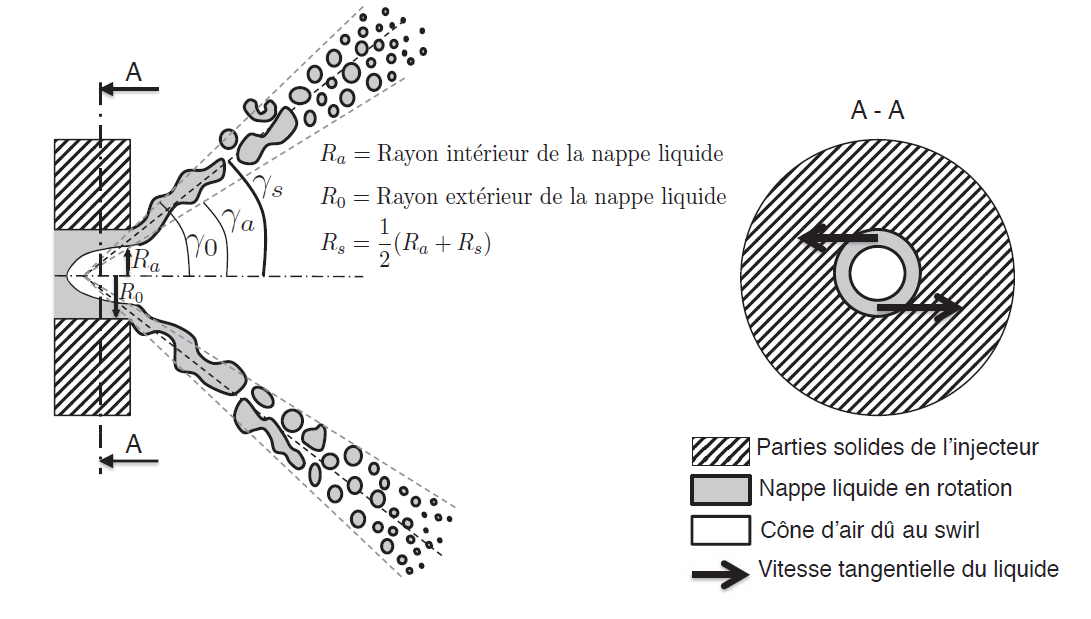
\includegraphics[width=0.8\textwidth]{./part1_numerical_approaches/figures_ch3/LISA}
       \centering
    \caption{LISA model for injection in pressure-swirl atomizers. Source: \citeColor[guedot_developpement_2015].}
    \label{fig:LISA_methodology}
\end{figure}




\subsection{Airblast spray}

In MSFI, at certain operating conditions the liquid injected through the pilot or take-off stages can impinge the walls of the atomizer forming an airblast spray. These have been extensively studied \citemColor[lefebvre_airblast_1980, gepperth_pre-filming_2010] and used in industrial burners, found in atomizers of type plain jet or prefilmers \citepColor[lefebvre_atomization_2017].

Regarding numerical approaches to simulate airblast sprays, a phenomenological model was derived by \citeColor[chaussonnet_new_2016] called PAMELA (Primary Atomization Model for prEfilming airbLAst injectors). This model uses results obtained in the KIT-ITS airblast experiment by \citeColor[gepperth_pre-filming_2010] for predicting initial conditions for droplets sizes and velocities. Correlations and laws for droplets sizes are derived by observing the breakup mechanisms found in airblast spray, shown in Figure \ref{fig:airblast_breakup_mechanism_chaussonnet}. This thesis does not address airblast atomization and hence this model is no longer discussed here: the interested reader is referred to \citeColor[chaussonnet_modeling_2014] and \citeColor[chaussonnet_new_2016] for more details into PAMELA model, and to \citeColor[carmona_modelisation_2021] for a more recent extention of this model, named Automatic-PAMELA, to a wider range of geometries and operating conditions. Other recent works aim at understanding the spray distribution from resolved calculations 


\begin{figure}[ht]
    \centering
    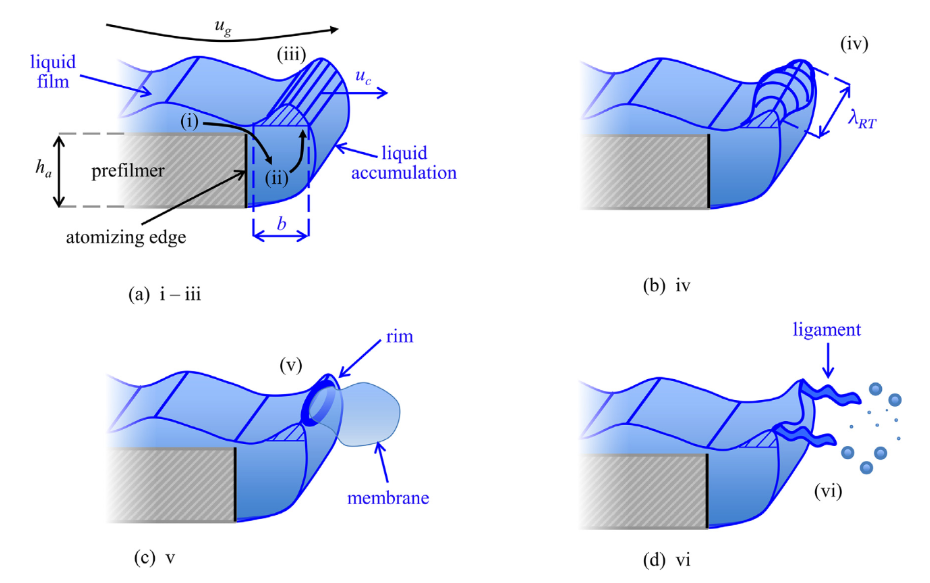
\includegraphics[width=0.9\textwidth]{./part1_numerical_approaches/figures_ch3/airblast_breakup_mechanism_chaussonnet}
       \centering
    \caption[Breakup mechanism in an airblast prefilmer spray]{Breakup mechanism in an airblast prefilmer spray. Source: \citeColor[chaussonnet_new_2016].}
    \label{fig:airblast_breakup_mechanism_chaussonnet}
\end{figure}




\subsection{Liquid jet in crossflow}
\label{ch3:subsec_lagrangian_liquid_JICF}

Several numerical approaches have been used to study liquid jet in crossflow injection, whose phenomenology has been introduced in $\S$\ref{sec:ch1_fuel_injection_technology}. Figure \ref{fig:jaegle_jicf_modeling_approaches} shows four different modeling approaches.  Case (a) is the direct simulation of the jet (resolved atomization computation) performed with the methodologies introduced in Chapter \ref{ch2:numerical_methods_resolved_atomization}, which has been used in several works  \citemColor[herrmann_detailed_2009,pai_role_2009,behzad_surface_2016,li_detailed_2018]. The other three approaches englobe several ways of tackling JICF simulations from a lagrangian perspective, where droplets are injected. All the categories from Figure \ref{fig:jaegle_jicf_modeling_approaches} take into account, one way or another, the liquid column (dense core) and hence its influence on the gaseous phase. This section reviews seven different past works to tackle liquid JICF from a lagrangian perspective. These works, which are all classified in Figure \ref{fig:state_art_injection}, are explained in chronological order. 

\clearpage

\begin{figure}[ht]
    \centering
    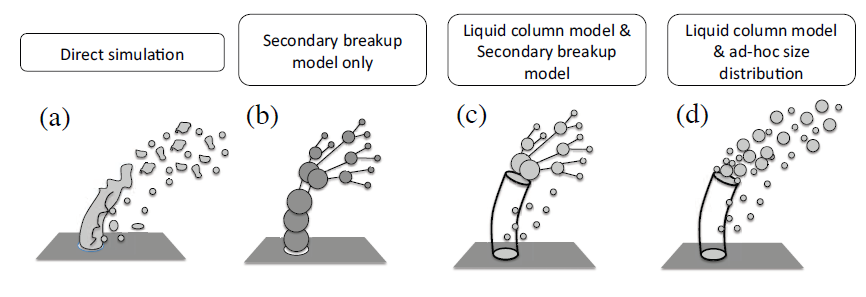
\includegraphics[width=1.0\textwidth]{./part1_numerical_approaches/figures_ch3/modelling_approaches_JICF_Jaegle}
       \centering
    \caption{Modeling approaches for liquid jet in crossflow proposed by \citeColor[jaegle_large_2009].}
    \label{fig:jaegle_jicf_modeling_approaches}
\end{figure}


\subsubsection*{Blob model combined with secondary atomization \citepBlackColor[apte_les_2003]}

%\citeColor[apte_les_2003] performed simulations of a water JICF. The objective of their work was to test a secondary atomization model in simulations representative of realistic gas-turbine configurations. The atomization model is described in Chapter 4 of this document. For performing injection, droplets with size of the nozzle diameter were introduced perpendicularly to the crossflow. Their velocity is the bulk liquid velocity at injection. This methodology is inspired on the blob model developed by \citeColor[reitz_modeling_1987], who simulated simulated diesel jets by injecting droplets of the diameter size which were later broke by action of a breakup model. 


\citeColor[apte_les_2003] performed simulations of a water JICF. The objective of their work was to test a secondary atomization model in simulations representative of realistic gas-turbine configurations. This breakup model is detailed in $\S$\ref{subsec:ch4_goro_model} of this document. For liquid injection, droplets with size equal to the nozzle diameter were introduced perpendicularly to the crossflow. Their velocity is the bulk liquid velocity at injection. This methodology is inspired by the blob model developed by \citeColor[reitz_modeling_1987], who simulated diesel jets by injecting droplets with size equal to the nozzle diameter which were later broken by action of an atomization model. 

The model by \citeColor[apte_les_2003] is included in the (b) category of Figure \ref{fig:jaegle_jicf_modeling_approaches}. Due to their initial big size, the droplets can easily influence the incoming gaseous flow field by means of two-way coupling between lagrangian particles and gas. Figure \ref{fig:apte_2003_jicf} shows the results obtained by \citeColor[apte_les_2003]. The jet leaving the nozzle is composed of large droplets. These particles bend towards the crossflow direction due to momentum exchange and break into smaller sizes due to the action of the secondary atomization model. The black and white contours denote the axial gas velocity profile at the central plane, showing the perturbation effect of the liquid onto the crossflow. This model presents the advantages that it is simple, cheap and does not rely on empirical correlations. On the other hand, the liquid column dynamics and breakup are not properly represented through the blob model. Consequently, the liquid-gas interaction is limited to only the two-way coupling and complex turbulent gas structures caused by the dense core are not captured, which could also influence secondary atomization.

\begin{figure}[ht]
    \centering
    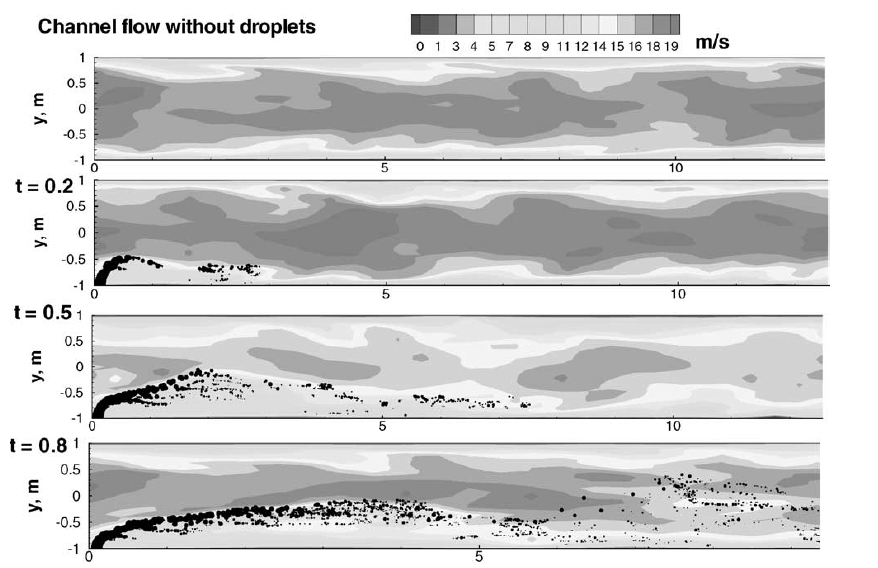
\includegraphics[width=0.75\textwidth]{./part1_numerical_approaches/figures_ch3/apte_2003_jicf}
       \centering
    \caption{Contours of instantenous axial velocity and liquid JICF evolution simulated by \citeColor[apte_les_2003].}
    \label{fig:apte_2003_jicf}
\end{figure}

\subsubsection*{Modeling the liquid-gas interaction with resolved dense core \citepBlackColor[arienti_aerodynamic_2006]}

\citeColor[arienti_aerodynamic_2006] focused their work on capturing the liquid-gas interaction between the liquid column and the gaseous crossflow. For this purpose, they combined a Volume-of-Fluid (VOF) method (see $\S$\ref{subsec:ch2_VOF} for a review on VOF) to solve for the dense core with a lagrangian approach to inject and transport droplets. By properly solving for the continuous liquid phase, the blockage effect is directly taken into account without the need of any extra models. Figure \ref{fig:arienti_2006_jicf} left shows front and side views (top and bottom, respectively) of the the dense core resolved by VOF (snapshot a) and of the mean gaseous vector fields at the same planes (snapshot b). Vortices created by the presence of the dense core are captured in both planes with this strategy, hence demonstrating its applicability to model the liquid-gas interaction.


\begin{figure}[ht]
    \centering
    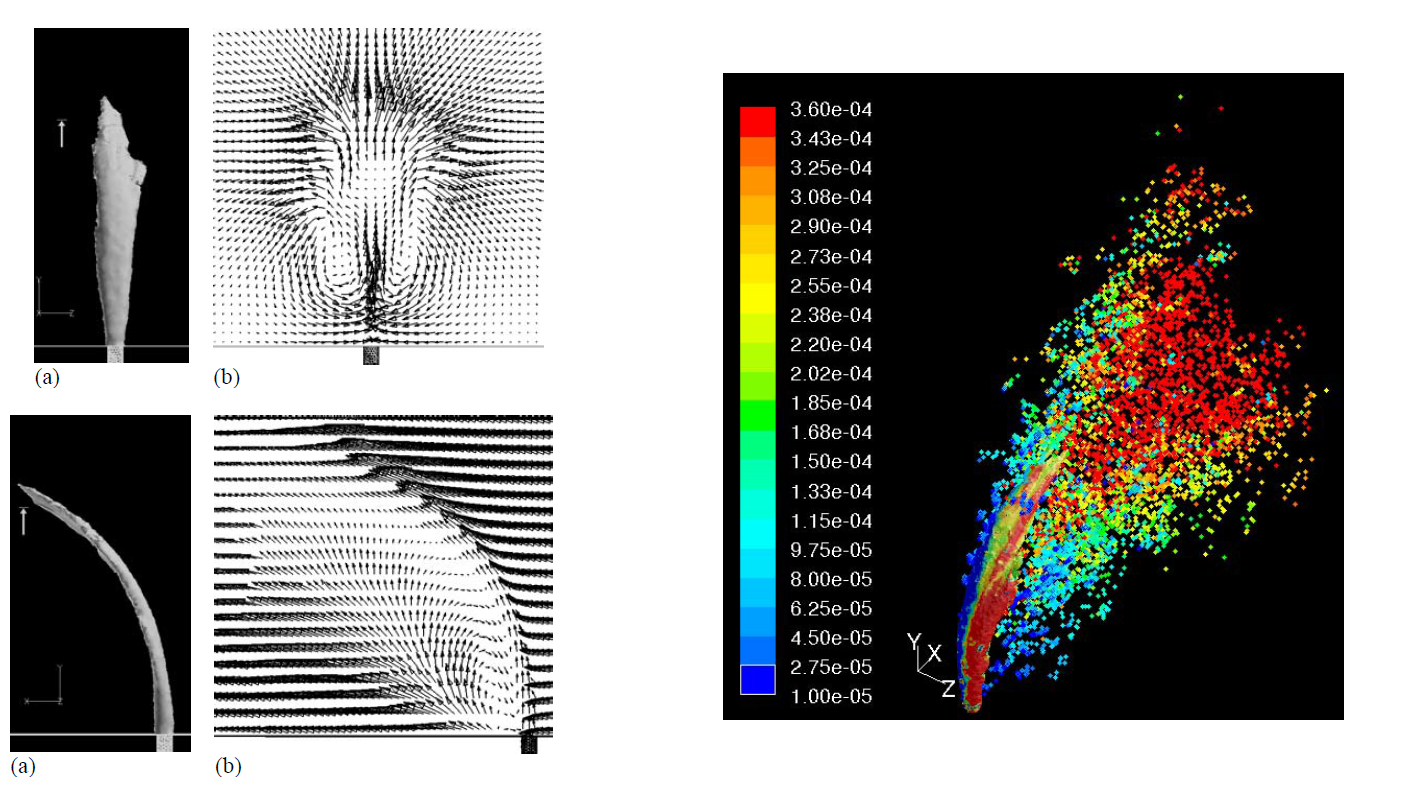
\includegraphics[width=0.8\textwidth]{./part1_numerical_approaches/figures_ch3/arienti_2006_jicf_ORIGINAL}
       \centering
    \caption[Jet in crossflow simulated with VOF plus lagrangian approach.]{Jet in crossflow simulated with VOF plus lagrangian approach. \textsl{Left}: dense core view and vector lines showing vortical structures. \textsl{Right}: instantaneous snapshot of droplets injected along the dense core. Source: \citeColor[arienti_aerodynamic_2006].}
    \label{fig:arienti_2006_jicf}
\end{figure}

Injection of lagrangian particles is performed at several locations alongside the liquid column, equally spaced between the nozzle exit and the column breakup point. Droplets sizes are obtained from experimental correlations, while the initial velocity is the continuous phase velocity (i.e. from the liquid column) at the same location plus a fluctuating component obtained as the product between a gaussian PDF and the local turbulent velocity from VOF. Figure \ref{fig:arienti_2006_jicf} right shows a instantaneous snapshot of the spray, depicting the dense core and the injected droplets colored by their diameter. Additional submodels considered in the computation include dispersion models to account for turbulent fluctuations during droplets transport \citepColor[gosman_aspects_1983] and the wave secondary atomization model developed by \citeColor[reitz_modeling_1987]. This model presents the advantage of directly accounting for the liquid dense core, hence capturing the complex liquid-gas interaction. On the other hand, it relies on empirical correlations to estimate the breakup location (which limits its application to the validity range of the experiments) and is computationally more expensive than a full lagrangian model, as it also solves for the dense core with the resolved method VOF.




\subsubsection*{Modeling column and shear breakup with empirical laws \citepBlackColor[jaegle_large_2009]}

At operating conditions corresponding to surface breakup (Figure \ref{fig:jicf_breakup_regime_wu}), there are small droplets being torn apart from the liquid column due to the high aerodynamic shear. The quantity of liquid removed by this mechanism is more notorious as $q$ and $We$ are larger. At the same time, there is also the liquid column which undergoes instabilities and breaks first into ligaments (primary atomization) and then into smaller droplets (secondary atomization). Figure \ref{fig:jaegle_senoner_modeling_strategies} left shows both mechanisms of droplet generation.

\begin{figure}[ht]
    \centering
    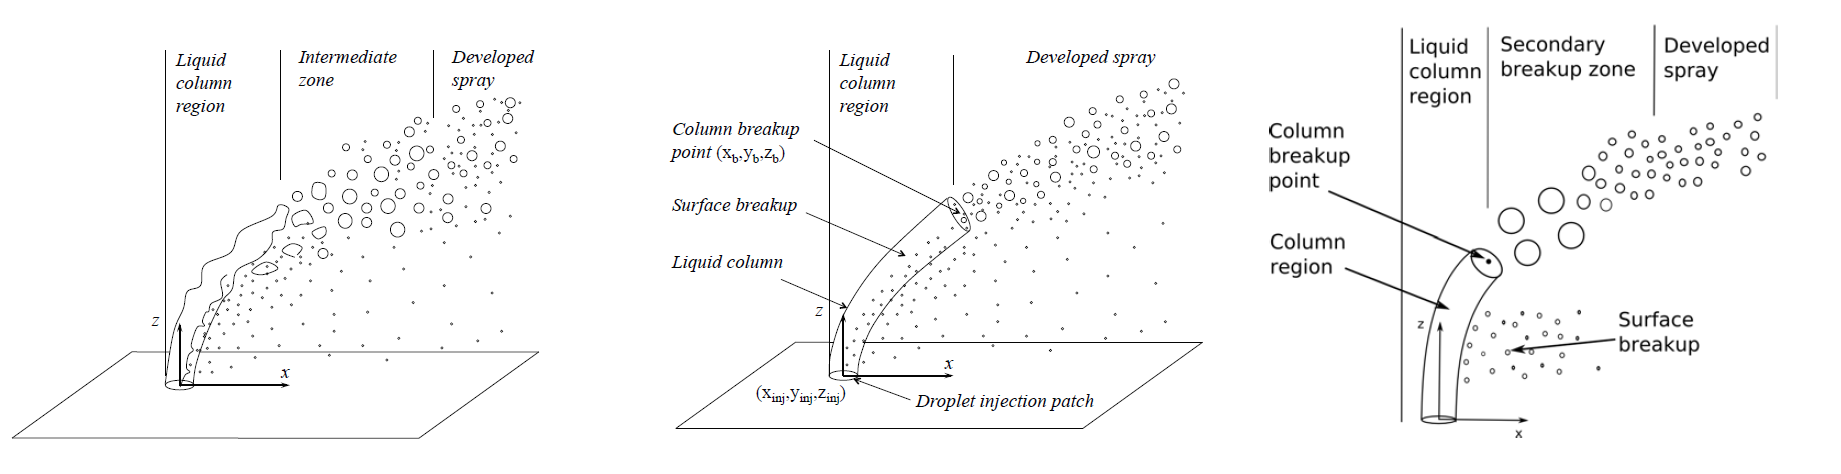
\includegraphics[width=1.0\textwidth]{./part1_numerical_approaches/figures_ch3/jaegle_senoner_modeling_strategies}
       \centering
    \caption[Schemes showing numerical models for liquid jets in crossflow]{Schemes showing numerical models for liquid jets in crossflow. \textsl{Left}: classification of different regions of the liquid jet atomization. \textsl{Center}:  column model considered by \citeColor[jaegle_large_2009], neglecting the intermediate zone and secondary breakup. \textsl{Right}: column model considered by  \citeColor[senoner_simulation_2010].}
    \label{fig:jaegle_senoner_modeling_strategies}
\end{figure}


Some numerical methodologies try to predict the size and flow rate of droplets generated by surface breakup, while simultaneously taking into consideration the liquid column. \citeColor[jaegle_large_2009] has used this strategy by using empirical laws to predict the liquid column, the size of the injected particles and the flow rate of droplets generated by surface breakup. His approach is illustrated in Figure \ref{fig:jaegle_senoner_modeling_strategies} center. Droplets are injected at the injection patch, which corresponds to the liquid nozzle exit. The liquid column is not resolved, but its region of influence is estimated in order to impose a modified drag law to the droplets that are convected within it. Once these droplets abandon the column region, the drag law is changed to the usual one. At the same time, there are droplets being injected along the liquid column region in the axial direction to model the surface breakup mechanism.




The first step in this model is to estimate the region to modify the drag law. For it, the liquid column is assumed to be cylindrical and to expand from the liquid nozzle exit until the breakup point $\left( x_\mathrm{b}, y_\mathrm{b}, z_\mathrm{b} \right)$. Its location is estimated from the following experimental expressions by \citeColor[fuller_effects_2000]:

\begin{subequations}
\label{eq:jaegle_breakup_point}
\begin{align}
\frac{x_b}{d_\mathrm{inj}} &= \frac{C_D C_{ab}^2}{\pi} \\
\frac{y_b}{d_\mathrm{inj}} &= 0 \\
\frac{z_b}{d_\mathrm{inj}} &= C_{ab} \frac{u_l}{u_\infty} \sqrt{\frac{\rho_l}{\rho_\infty}}
\end{align}
\end{subequations}

where $C_D = 4.39$ is a constant drag coefficient, $C_{ab} = 2.58$ is a breakup coefficient, $u_l$ is the liquid velocity at injection and $u_\infty$ is the gas freestream velocity. The particles travelling in the liquid column region will follow the following modified transport law \citepColor[fuller_effects_2000]:

\begin{subequations}
\label{eq:momentum_jaegle_model}
\begin{align}
\frac{d u_l}{d t} &= \frac{2 C_D}{d_\mathrm{inj} \pi} \frac{\rho_l}{\rho_\infty} \left( u_\infty - u_l \right)^2  \\
\frac{d v_l}{d t} &= 0 \\
\frac{d w_l}{d t} &= 0 
\end{align}
\end{subequations}

Particles are injected at the liquid nozzle exit with velocity $u_l$ and a size sampled from a distribution obtained experimentally by \citeColor[becker_breakup_2002]. Simultaneously, stripped-off droplets are injected at random locations along the liquid column to account for surface breakup. The mass flow rate $\dot{m}_{l,SB}$ and constant size $SMD_{SB}$ of these droplets are given by the experimental expressions of \citeColor[ranger_aerodynamics_1968] and \citeColor[chou_temporal_1997], respectively:

\begin{subequations}
\label{eq:surface_breakup_jaegle_model}
\begin{align}
\dot{m}_{l,SB} &= \frac{3}{2} l_\mathrm{col} \rho_l \sqrt{\pi d_\mathrm{inj}} A a_l u_\infty \\
SMD_{SB} &= 0.09 d_\mathrm{inj} \\
u_{l,SB} &= u_c + 0.37 \left( u_\infty - u_c \right)
\end{align}
\end{subequations}

where $l_\mathrm{col}$ is the length of the liquid column, $u_c$ is the streamwise velocity of liquid column at the location of surface breakup, and $A$ and $a_l$ are constants obtained from the fluid properties and operating conditions \citepColor[ranger_aerodynamics_1968]. An example of the simulated lagrangian JICF obtained by \citeColor[jaegle_large_2009] is shown in the top of Figure \ref{fig:jaegle_senoner_lagrangian_fields}. This model presents the advantage that it is computationally cheap and, despite directly injecting a developed spray, it models the drag effects created by the liquid column and the shear stripping phenomenon through empirical laws. On the other hand, it is only applicable to the operating condition for which the experimental laws and the prescribed size distribution were obtained (high Reynolds numbers), and does not capture the complex liquid-gas interactions created by the liquid column.

\begin{figure}[ht]
    \centering
    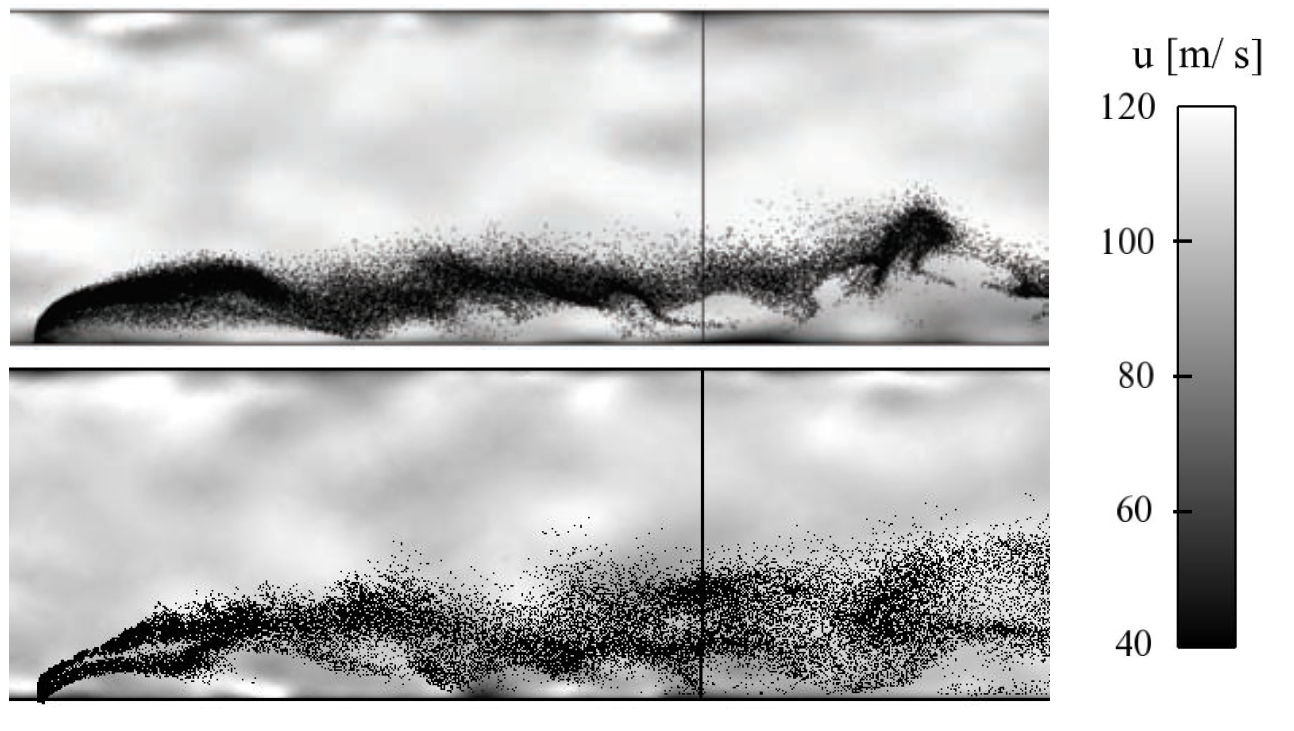
\includegraphics[width=0.6\textwidth]{./part1_numerical_approaches/figures_ch3/jaegle_senoner_lagrangian_fields}
       \centering
    \caption[Instantaneous axial gaseous velocity field on the plane y = 0 mm together with the lagrangian
droplets.]{Instantaneous axial gaseous velocity field on the plane y = 0 mm together with the lagrangian
droplets. q = 6. \textsl{Top}: numerical results by \citeColor[jaegle_large_2009]. \textsl{Bottom}: numerical results by \citeColor[senoner_simulation_2010].}
    \label{fig:jaegle_senoner_lagrangian_fields}
\end{figure}

\subsubsection*{Combining shear breakup with blob method and secondary atomization \citepBlackColor[senoner_simulation_2010]}

A similar approach to the previous one has been explored by \citeColor[senoner_simulation_2010]. In the same way as \citeColor[jaegle_large_2009] (and in the same experimental configuration), the breakup point is calculated from Eqs. (\ref{eq:jaegle_breakup_point}). This location defines then the column region where the modified law of Eqs. (\ref{eq:momentum_jaegle_model}) is applied. Regarding surface breakup, the same methodology employed by \citeColor[jaegle_large_2009] (previous model discussed) is followed, where droplets are injected with the properties given in Eqs. (\ref{eq:surface_breakup_jaegle_model}).

The originality of the approach by \citeColor[senoner_simulation_2010] lies on the size of particles at injection. While the previous model injects a developed spray, the current one introduces droplets with constant size through the liquid nozzle. The prescribed droplet's diameter is determined by the following expression: %Eq. (\ref{eq:ch5_senoner_model_ddrop}):

\begin{equation}
\label{eq:ch5_senoner_model_ddrop}
d_\mathrm{drop} = \sqrt[3]{\frac{3}{2} d_\mathrm{inj} \lambda_s}
\end{equation}

where $\lambda_s \approx 0.15 d_\mathrm{inj}$ is the wavelength of the column surface instabilities \citepColor[sallam_breakup_2004]. These droplets will then break into smaller ones through a secondary atomization model \citepColor[apte_les_2003]. The present model can be illustrated as in Figure \ref{fig:jaegle_senoner_modeling_strategies} right. A snapshot of the lagrangian jet obtained by this methodology is shown in Figure \ref{fig:jaegle_senoner_lagrangian_fields} bottom. This model has the same advantages as the one by \citeColor[jaegle_large_2009] (i.e. computationally cheap, drag effects by dense core are modeled, shear stripping of droplets is considered), plus it accounts for secondary breakup and does not rely on experimental particles size distributions. On the other hand, it also needs empirical laws for modeling particles' drag at the dense core region and the shear stripping phenomenon (valid at high Reynolds number), and it does not capture the complex liquid-gas interactions created by the liquid column.




\subsubsection*{Semi-empirical model for shear breakup regime \citepBlackColor[eckel_semi-empirical_2016]}

Following the line of modeling shear breakup, \citeColor[eckel_semi-empirical_2016] developed a semi-empirical model for this regime. The numerical strategy is depicted in Figure \ref{fig:eckel_2016_modeling_strategy}. This approach injects cylindrical parcels (a,b) mimicking the dense structures of the liquid column which are tracked with a lagrangian formalism and transported with a modified drag law (c). These cylinders have the same diameter as the injection orifice.  As the parcels move, droplets modeling shear breakup are stripped-off the column (d) with properties (mass flow rate, sizes, velocities) given by experimental laws (e). The parcels will then lose mass until they reach a residence time corresponding to the breakup of the liquid column (f), when they are broken into smaller, spherical droplets representing column breakup (g). This approach is continuously performed to model the jet behaviour (h). Dispersion models are used for enhancing the droplet transport \citepColor[gosman_aspects_1983]. Models to account for secondary breakup are not needed, as the employed approach generates a developed spray. A snapshot of the resulting jet is shown in Figure \ref{fig:eckel_2016_jet}, where the difference between the liquid column made of cylindrical parcels and the developed spray zone composed by spherical droplets is clearly visible. The advantages of this method are its low computational cost and its consideration of complex physical phenomena such as liquid column drag, shear stripping, primary and secondary atomization. On the other hand, this model is exclusively built on empirical laws which are valid for Weber numbers (We) corresponding to the shear breakup regime, making it unapplicable to higher We regimes (catastrophic breakup) or lower ones (bag breakup).


\begin{figure}[ht]
    \centering
    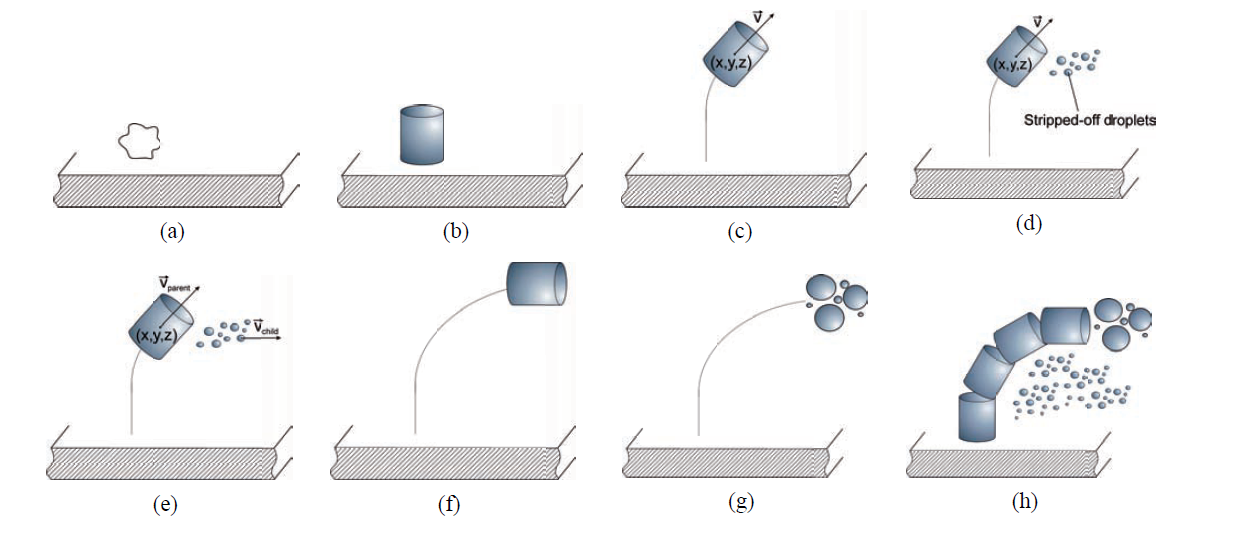
\includegraphics[width=1.0\textwidth]{./part1_numerical_approaches/figures_ch3/eckel_2016_modeling_strategy}
       \centering
    \caption{Jet in crossflow modeling strategy followed by \citeColor[eckel_semi-empirical_2016].}
    \label{fig:eckel_2016_modeling_strategy}
\end{figure}



\begin{figure}[ht]
    \centering
    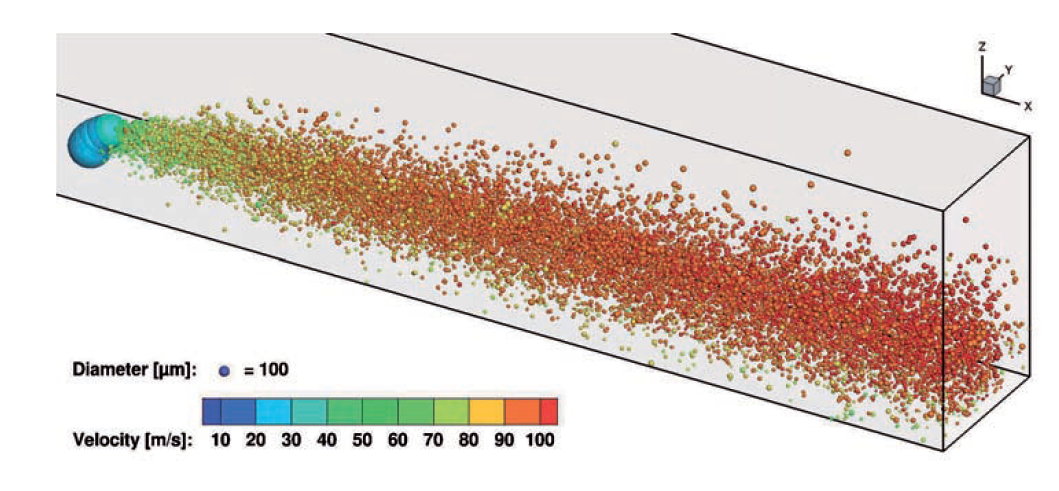
\includegraphics[width=0.6\textwidth]{./part1_numerical_approaches/figures_ch3/eckel_2016_jet}
       \centering
    \caption{Simulation of jet in crossflow by \citeColor[eckel_semi-empirical_2016].}
    \label{fig:eckel_2016_jet}
\end{figure}


\subsubsection*{Statistical method for injection of a fully developed spray \citepBlackColor[fan_eulerianlagrangian_2018]}

All the methodologies previously discussed, except for \citeColor[arienti_aerodynamic_2006], performed injection of droplets at the nozzle orifice center with the liquid injection velocity. Furthermore, large droplets of the order of the nozzle diameter were injected in all cases except in the model of \citeColor[jaegle_large_2009], who introduced a developed spray. In this line, the work of \citeColor[fan_eulerianlagrangian_2018] explored an approach to inject a developed spray at the nozzle orifice following a statistical method. Each particle is injected with attributes chosen as follows:

\begin{itemize}
	
	\item Diameter: sampled from a Probability Density Function (PDF) $f \left(  D \right)$. Four PDFs for droplet sizes were studied: uniform, $\upchi^2$, Nukiyama-Tanasawa and Rosin-Rammler.

	\item Velocity: randomly chosen from a Gaussian distribution with standard deviation equal to the liquid injection velocity.
	
	\item Injection location: at a random point in a circular patch placed at the liquid nozzle exit.

\end{itemize}

Figure \ref{fig:fan_2018_jets_penetration} shows a lateral view of the sprays and the penetration for four cases, each one injecting a different PDF for the droplet diameter. Each PDF gives a different range of droplet diameters and a different spray penetration, showing the importance of chosen accurately the initial boundary conditions for reproducing sprays with lagrangian formalism. This model presents the advantages of its simplicity (it defines the injection parameters according to mathematical expressions) and its low computational cost. On the other hand, the injection parameters have been calibrated with experimental results, hence this model cannot be applied without data for such calibration, and the liquid-gas interactions created by the liquid column are not modeled.

\begin{figure}[ht]
    \centering
    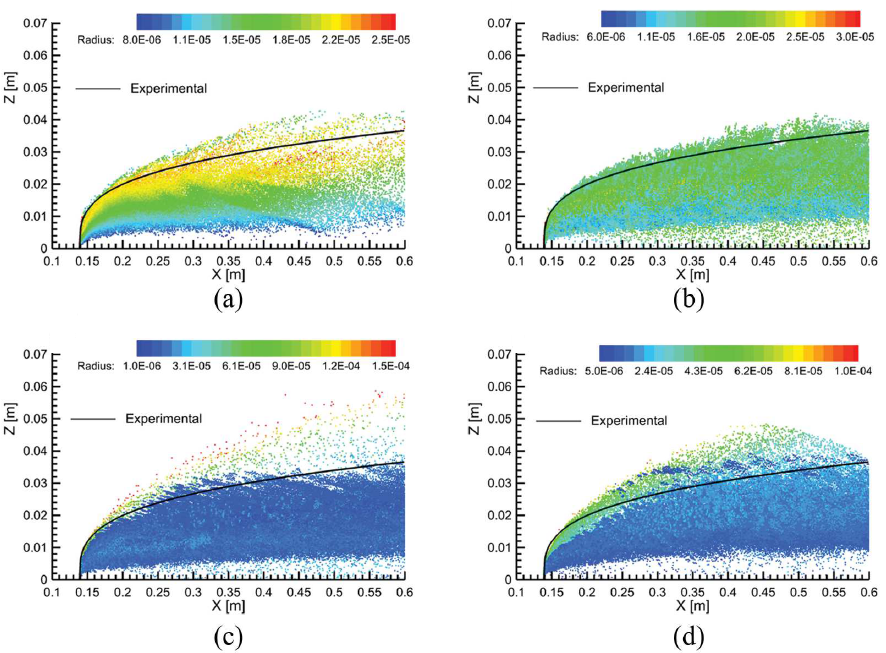
\includegraphics[width=0.7\textwidth]{./part1_numerical_approaches/figures_ch3/fan_2018_jets_penetration}
       \centering
    \caption{JICF sprays and penetrations obtained by \citeColor[fan_eulerianlagrangian_2018] with different injected PDFs for the droplets sizes. (a) Uniform distribution (b) $\upchi^2$ distribution (c) Nukiyama-Tanasawa distribution (d) Rosin-Rammler distribution.}
    \label{fig:fan_2018_jets_penetration}
\end{figure}



\subsubsection*{Hybrid model for jet in crossflow injection \citepBlackColor[fontes_improved_2019]}

One of the most recent works (up to date) focused on JICF modeling has been performed by \citeColor[fontes_improved_2019]. As in the study by \citeColor[arienti_aerodynamic_2006], this approach combines a direct resolution method (VOF) for solving the liquid column with an injection procedure for lagrangian droplets. Experimental correlations are used to obtain column breakup location. The liquid-gas interaction due to the dense core presence is therefore taken into account (Figure \ref{fig:fontes_2019_lagrangian_fields} left). Injection of lagrangian droplets is performed at the column breakup location (Figure \ref{fig:fontes_2019_lagrangian_fields} right): their velocity is equal to the liquid eulerian velocity at this point and their size is obtained from experimental correlations. Two operating points at low $We$ were simulated with this methodology, surface breakup was not modeled since it was not present at these conditions. This model presents the main advantage that it accounts for complex physical phenomena: secondary atomization, coalescence and complex liquid-gas interaction. On the other hand, it relies on empirical correlations obtained at low Weber numbers for determining the breakup coordinates, and neglects the shear stripping; hence, it is not suitable for application at high Weber numbers.

\clearpage

\begin{figure}[ht]
    \centering
    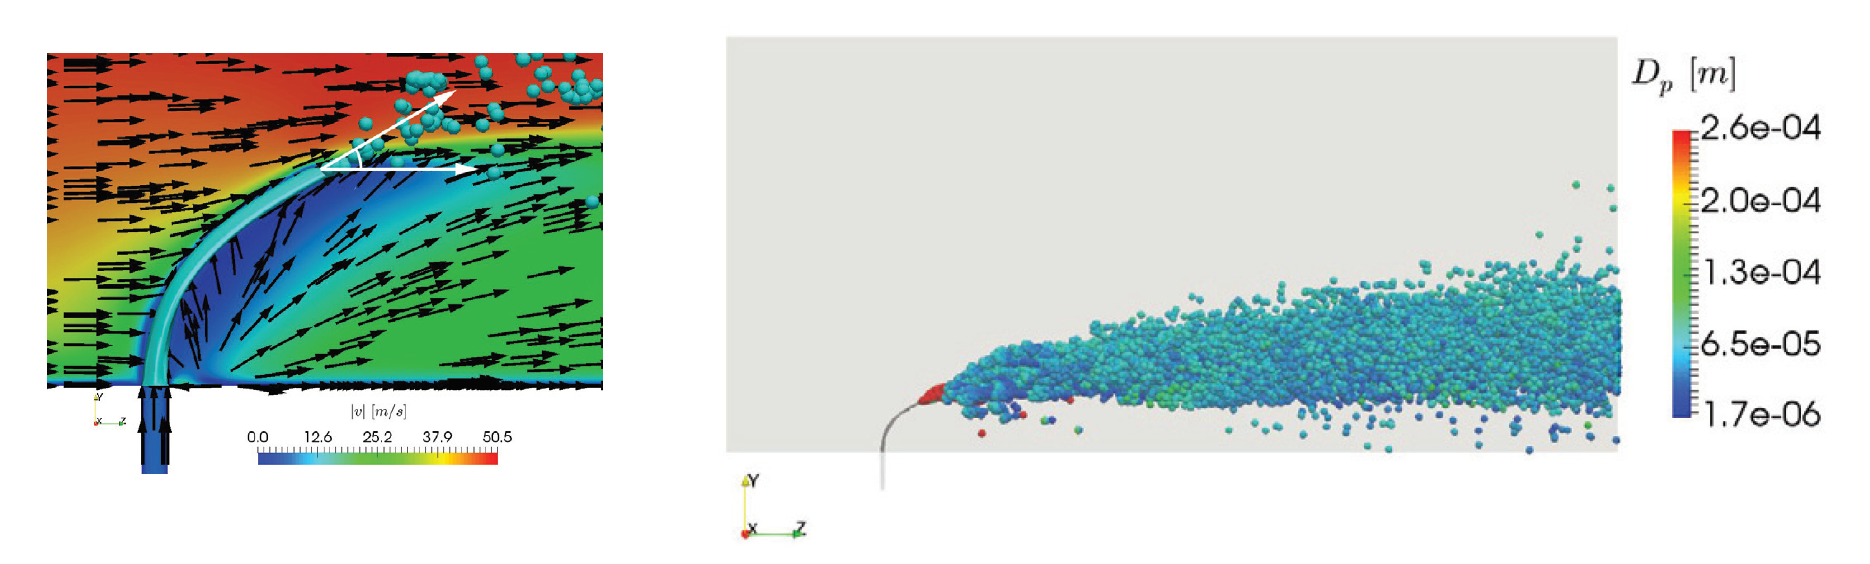
\includegraphics[width=0.9\textwidth]{./part1_numerical_approaches/figures_ch3/fontes_2019_lagrangian_fields}
       \centering
    \caption{Simulated jet in crossflow by \citeColor[fontes_improved_2019]. \textsl{Left}: close view of the near-jet, showing the resolved dense core with VOF and the perturbation effect on the gaseous field. \textsl{Right}: Farfield view of the jet, showing injection point of lagrangian droplets. Droplets are colored by their diameter. }
    \label{fig:fontes_2019_lagrangian_fields}
\end{figure}

 